% Welcome! This is the unofficial University of Udine beamer template.

% See README.md for more informations about this template.

% This style has been developed following the "Manuale di Stile"
% (Style Manual) of the University of Udine. You can find the
% manual here: https://www.uniud.it/it/ateneo-uniud/ateneo-uniud/identita-visiva/manuali-immagine-stile/manuale-stile

% Note: for some reason, the RGB values specified in the manual
% do NOT render correctly in Beamer, so they have been redefined
% for this document using the high level chromo-optic deep neural 
% quantistic technology offered by Microsoft Paint's color picker.

% We defined four theme colors: UniBrown, UniBlue, UniGold
% and UniOrange. For example, to write some uniud-brownish
% text, just use: \textcolor{UniBrown}{Hello!}

% Note that [usenames,dvipsnames] is MANDATORY due to compatibility
% issues between tikz and xcolor packages.

\documentclass[usenames,dvipsnames]{beamer}
\usepackage[utf8]{inputenc}
\usepackage{verbatim}
\usepackage{multicol}
\usepackage{cases}
\usepackage{multirow}
\usepackage{adjustbox}
\usepackage{cancel}
\usetheme{uniud}
%set depth of Outline
\setcounter{tocdepth}{2}
%%% Bibliography
\usepackage[style=authoryear,backend=biber]{biblatex}
\addbibresource{bibliography.bib}

%cancel the table of content before section
\AtBeginSection[]{}

% Author names in publication list are consistent 
% i.e. name1 surname1, name2 surname2
% See https://tex.stackexchange.com/questions/106914/biblatex-does-not-reverse-the-first-and-last-names-of-the-second-author
\DeclareNameAlias{author}{first-last}

%%% Suppress biblatex annoying warning
\usepackage{silence}
\WarningFilter{biblatex}{Patching footnotes failed}

%%% Some useful commands
% pdf-friendly newline in links
\newcommand{\pdfnewline}{\texorpdfstring{\newline}{ }} 
% Fill the vertical space in a slide (to put text at the bottom)
\newcommand{\framefill}{\vskip0pt plus 1filll}


\title[$Z\rightarrow \tau\tau$ modeling C1N2ISR, had-had channel]{$Z\rightarrow \tau\tau$ modeling\\ C1N2ISR, had-had channel}
\date[Jun 26, 2025]{Jun 26, 2025}
\author[Chengxin Liao]{
  Chengxin Liao
  \pdfnewline
  \texttt{liaocx@ihep.ac.cn}
}
\institute{Department of Physics, Shandong University}

\begin{document}

\begin{frame}
\titlepage
\end{frame}

%\begin{frame}{Outline}
%\tableofcontents
%\end{frame}

\section{HH channel Selection}
%\subsection{event selection}
\begin{frame}

\frametitle{HH channel Selection}
\begin{columns}
    \column{0.6\textwidth}
    \raggedright
    Selection
	\begin{enumerate}[\textbullet]
    
    \item nTaus$\geq$2
    
    \item nBaseLeps=0
    
    \item pass MET trigger; MET$\geq$ 200
    
    \item $1\leq nBaseJet$
     
    \item b-veto
    
    \item OS
    
    \item jet pt > 100GeV
    
    \item 40 $\leq$ reco $M_{tt}$ $\leq$ 130
    
    \end{enumerate}
    \vskip 0.2cm
    
Run 2 includes the 1516, 17 and 18 samples.

Run 3 includes the 22 and 23 samples.
%    For sig/bkg plot, both bkg and signal distribution are normalized to 1.
%    

%    
%    Kinematic variables with better separation power are marked with black box.
    \column{0.5\textwidth}
    
    \raggedleft
    \begin{figure}
    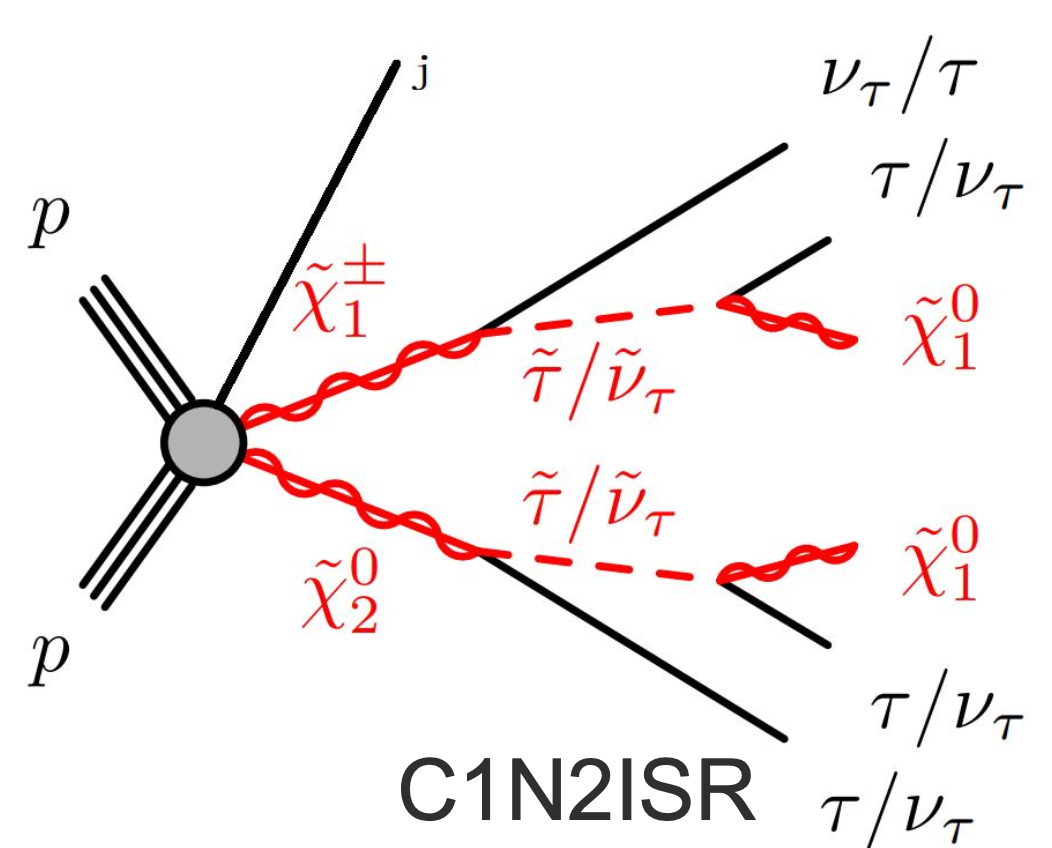
\includegraphics[width = 0.7\textwidth]{graphics/Feynman diagram.png}
    \end{figure}
 \end{columns}

\end{frame}

\begin{frame}
\frametitle{Yield Comparison: Run2 vs Run3}
\scriptsize
\centering

% ---- Z+jets Sample Table ----
\vspace{-0.5em}
\begin{tabular}{|c|l|l|}
\hline
\textbf{Type} & \textbf{dsid} & \textbf{Sample} \\
\hline
\multirow{2}{*}{Z+jets} 
  & 700792--700794,\quad 700901--700903 & Sh\_2214\_Ztautau\_maxHTpTV2 \\
  & 700360(only for run2) & Sh\_2211\_Ztt2jets\_Min\_N\_TChannel \\
\hline
\end{tabular}

\vspace{1em}

% ---- Yield Comparison Table ----
\begin{tabular}{|l|c|c|}
\hline
\textbf{Process} & \textbf{Run2 Yields} & \textbf{Run3 Yields} \\
\hline
Wjets          & 89.0 $\pm$ 12.0     & 50.33 $\pm$ 3.44     \\
Zlljets        & 0.07 $\pm$ 0.04     & 0.06 $\pm$ 0.02      \\
Zttjets        & 1323.75 $\pm$ 5.92  & 468.88 $\pm$ 3.11    \\
VV             & 49.77 $\pm$ 0.81    & 20.49 $\pm$ 0.36     \\
Top            & 25.35 $\pm$ 1.91    & 13.71 $\pm$ 1.12     \\
Higgs          & 16.5 $\pm$ 3.28     & --                   \\
dijet          & 24.03 $\pm$ 22.32   & 0.48 $\pm$ 0.37      \\
\hline
bkg wo dijet   & 1504.44 $\pm$ 13.93 & 553.47 $\pm$ 4.79    \\
bkg            & 1528.46 $\pm$ 26.31 & 553.95 $\pm$ 4.80    \\
data           & 1635.0 $\pm$ 40.44  & 712.0 $\pm$ 26.68    \\
\hline
\textbf{Ztt purity (wo dijet)} & \textbf{0.88} & \textbf{0.85} \\
\hline
\end{tabular}

\end{frame}



\section{Kinematic plots, run2}
\begin{frame}
	\frametitle{Kinematic plots, run2}
	
\makebox[\textwidth]{%
\begin{tabular}{ccccc}
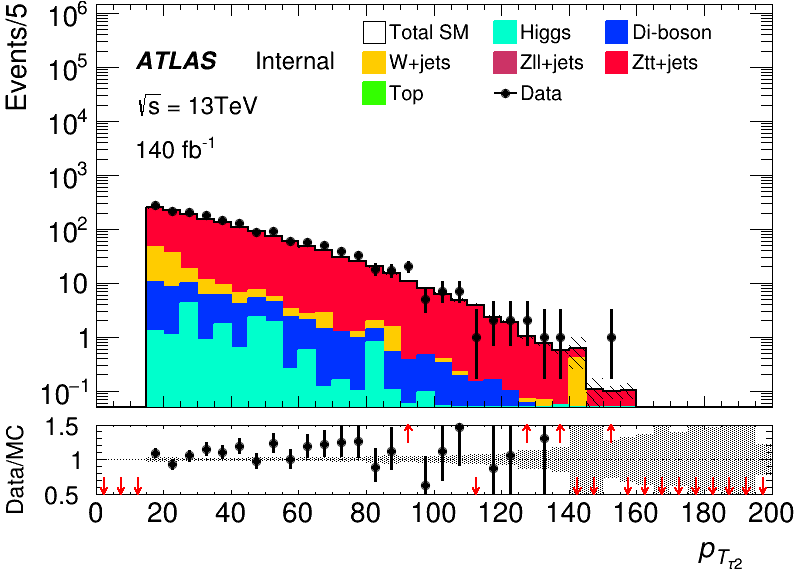
\includegraphics[width=0.20\textwidth]{graphics/HH_run2/HH_met_fb_pt_tau2.png} &
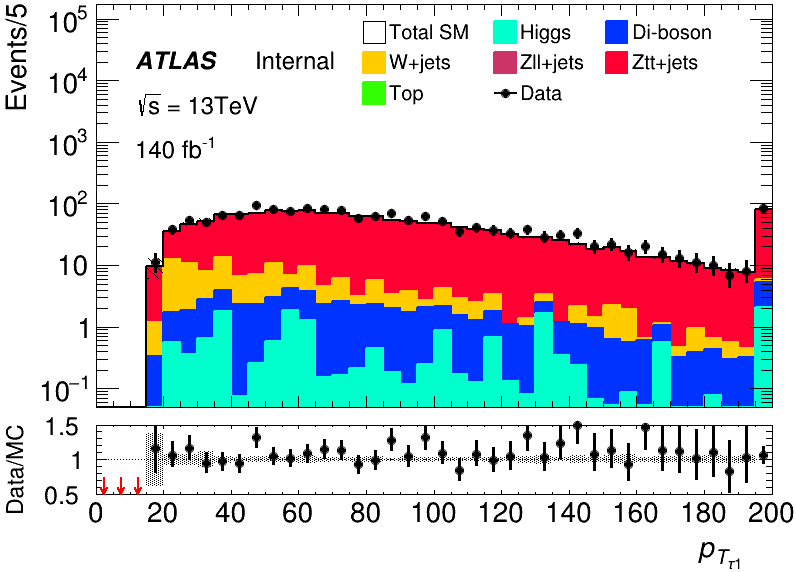
\includegraphics[width=0.20\textwidth]{graphics/HH_run2/HH_met_fb_pt_tau1.png} &
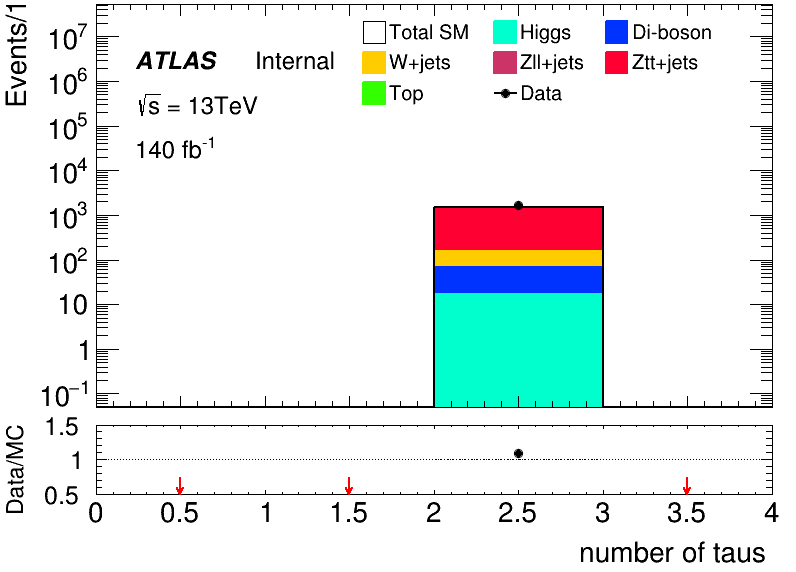
\includegraphics[width=0.20\textwidth]{graphics/HH_run2/HH_met_fb_nTaus.png} &
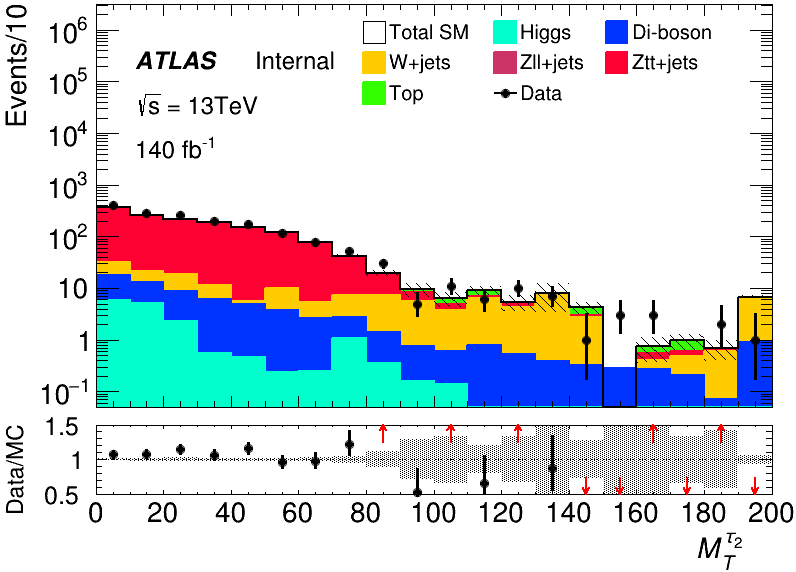
\includegraphics[width=0.20\textwidth]{graphics/HH_run2/HH_met_fb_mtx_tau2.png} &
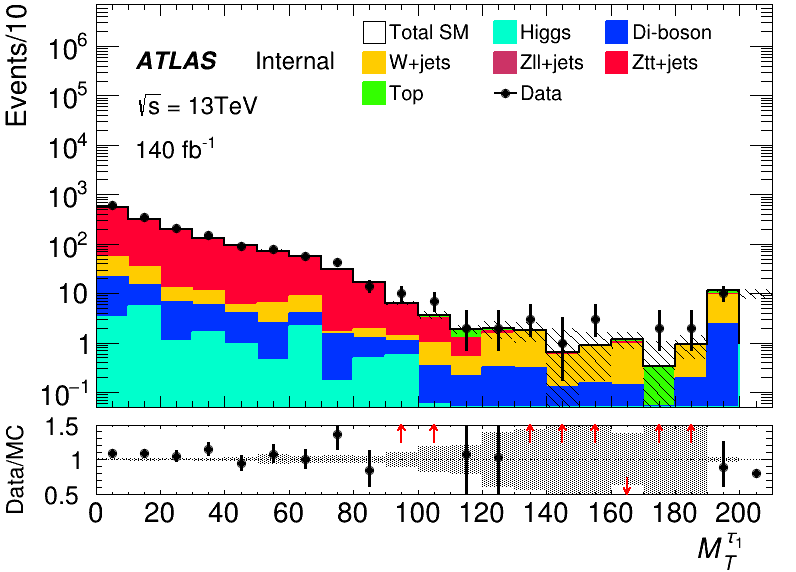
\includegraphics[width=0.20\textwidth]{graphics/HH_run2/HH_met_fb_mtx_tau1.png} \\
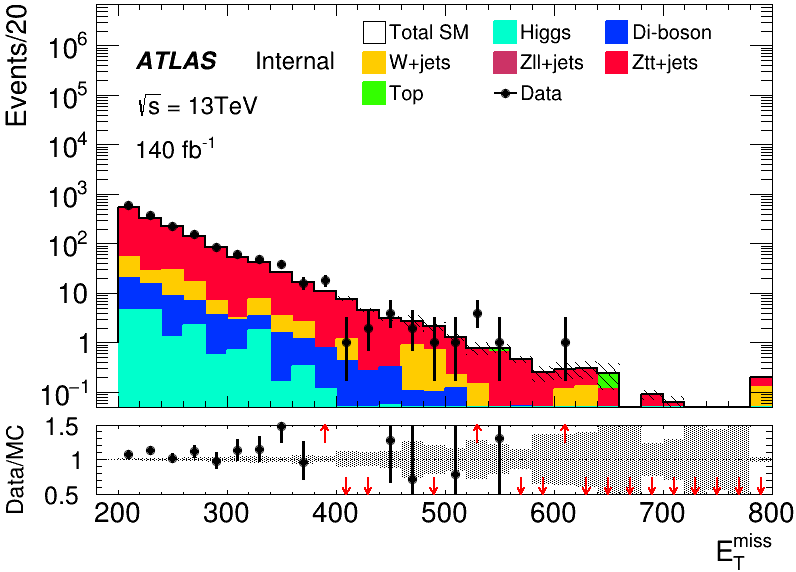
\includegraphics[width=0.20\textwidth]{graphics/HH_run2/HH_met_fb_MET.png} &
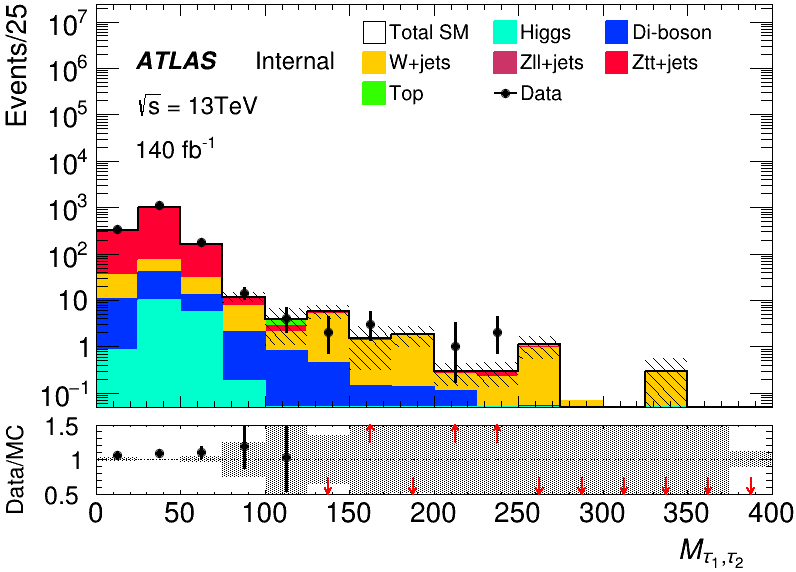
\includegraphics[width=0.20\textwidth]{graphics/HH_run2/HH_met_fb_Mll.png} &
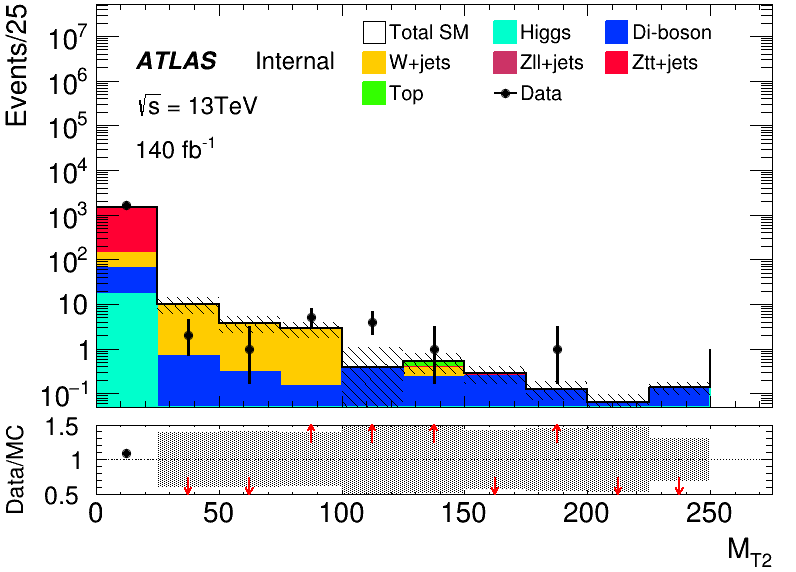
\includegraphics[width=0.20\textwidth]{graphics/HH_run2/HH_met_fb_MT2.png} &
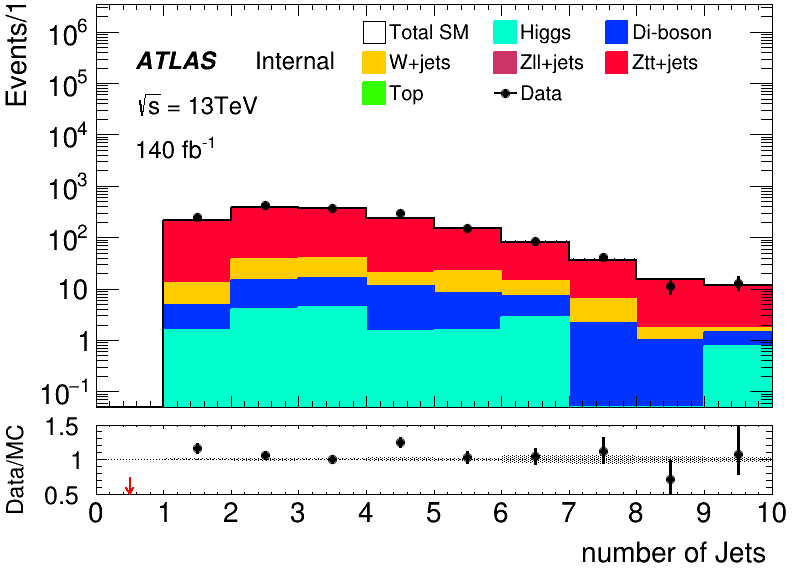
\includegraphics[width=0.20\textwidth]{graphics/HH_run2/HH_met_fb_nJets.png} &
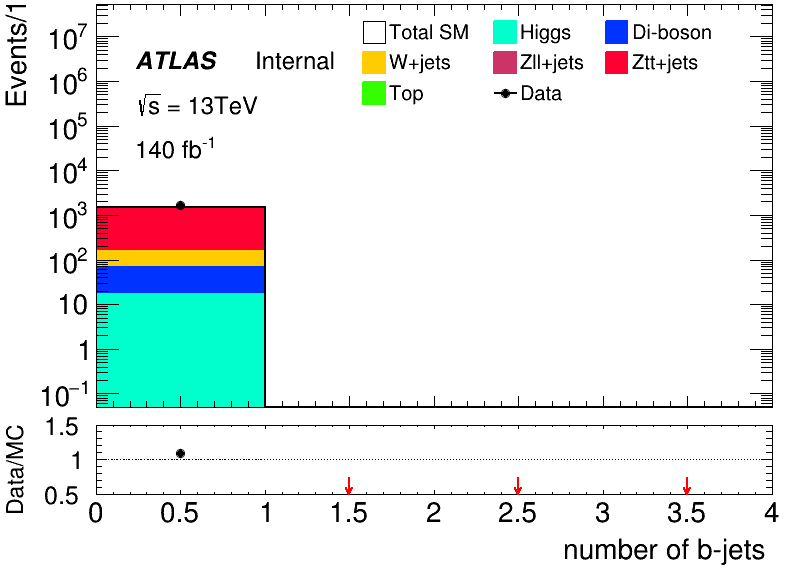
\includegraphics[width=0.20\textwidth]{graphics/HH_run2/HH_met_fb_bNumber.png} \\
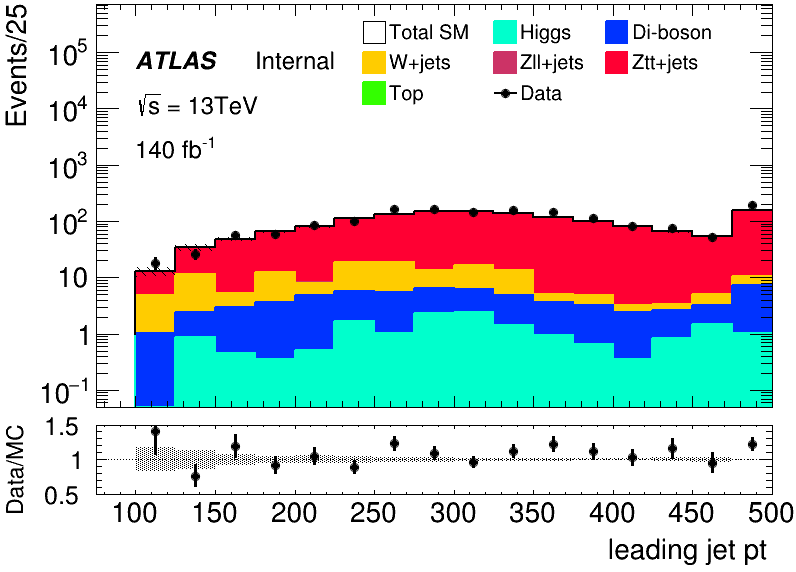
\includegraphics[width=0.20\textwidth]{graphics/HH_run2/HH_met_fb_pt_jet1.png} &
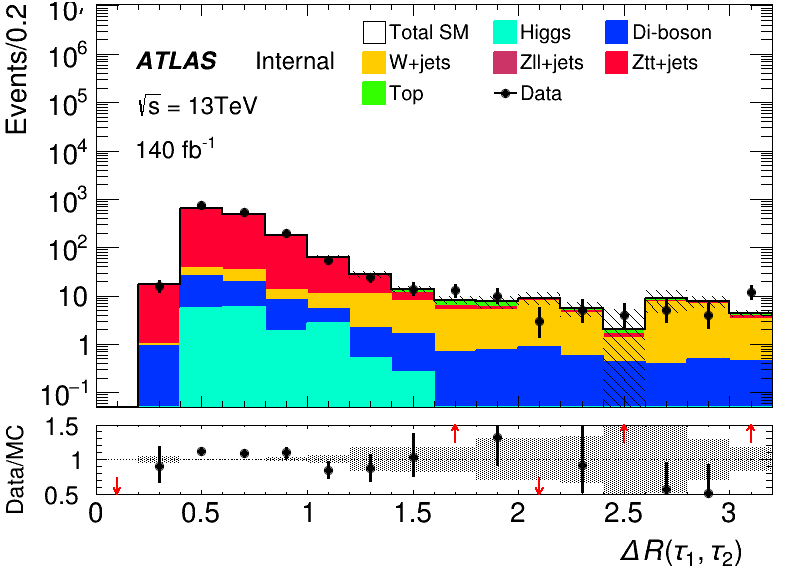
\includegraphics[width=0.20\textwidth]{graphics/HH_run2/HH_met_fb_dRtt.png} &
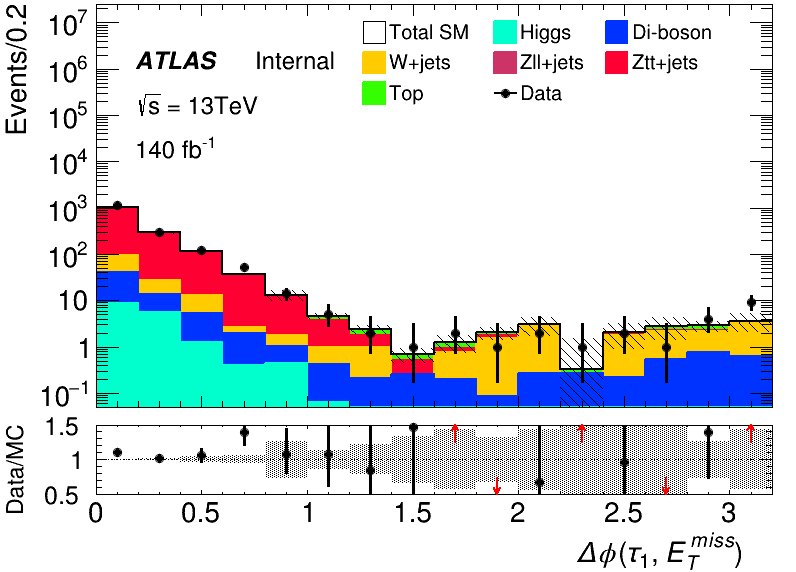
\includegraphics[width=0.20\textwidth]{graphics/HH_run2/HH_met_fb_dPhit1x.png} &
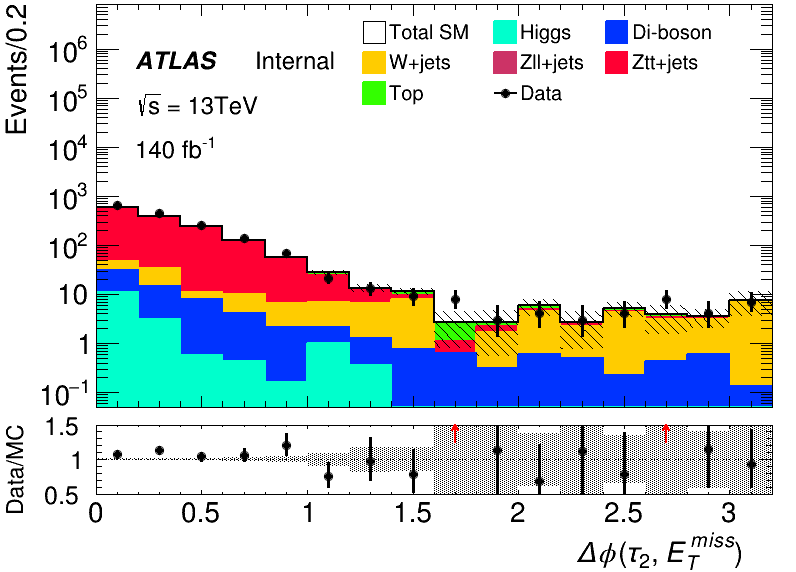
\includegraphics[width=0.20\textwidth]{graphics/HH_run2/HH_met_fb_dPhit2x.png} &
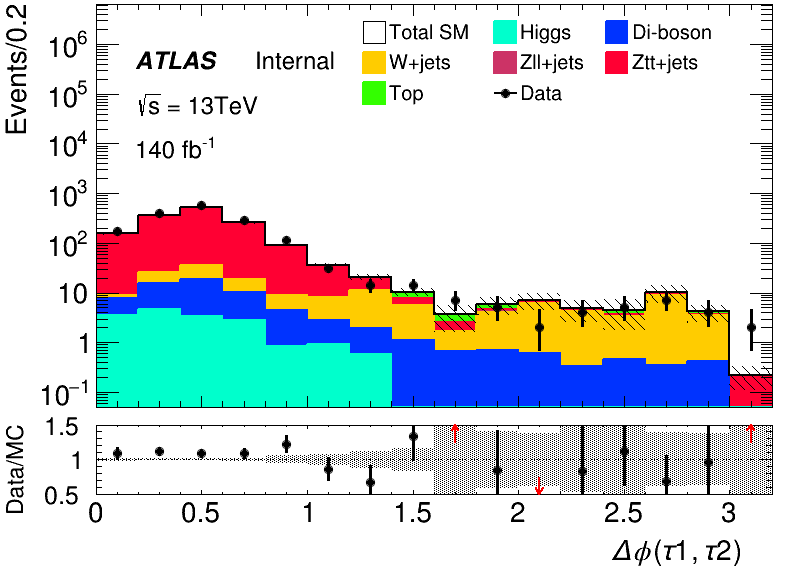
\includegraphics[width=0.20\textwidth]{graphics/HH_run2/HH_met_fb_dPhitt.png}
\end{tabular}
}

\end{frame}


\section{Kinematic plots, run3}
\begin{frame}{Kinematic plots, run3}

\makebox[\textwidth]{%
\begin{tabular}{ccccc}
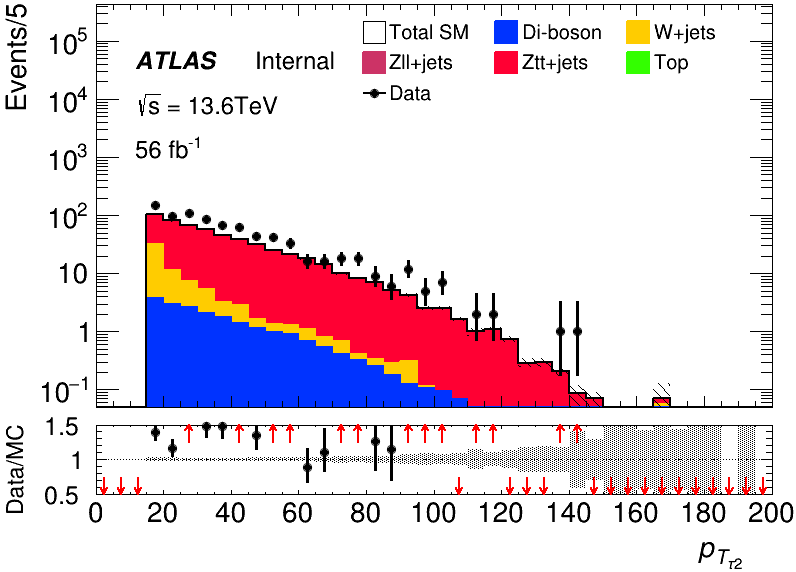
\includegraphics[width=0.20\textwidth]{graphics/HH_run3/HH_met_fb_pt_tau2.png} &
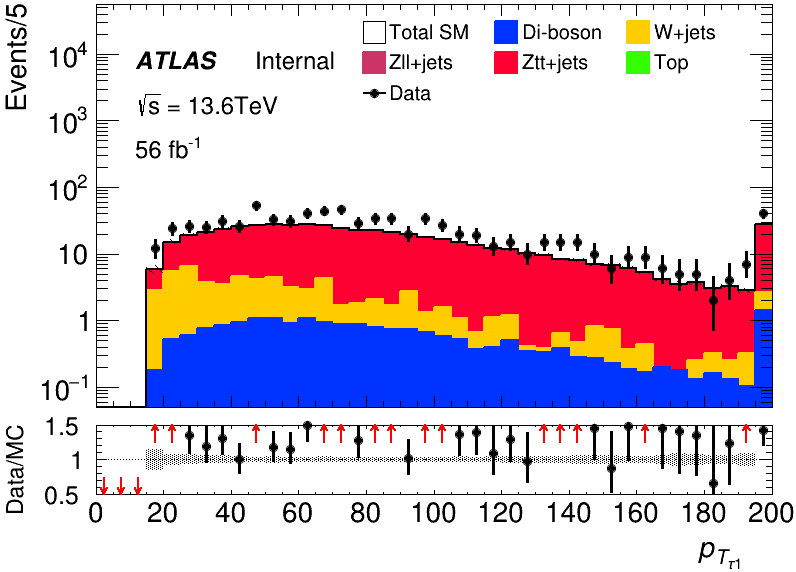
\includegraphics[width=0.20\textwidth]{graphics/HH_run3/HH_met_fb_pt_tau1.png} &
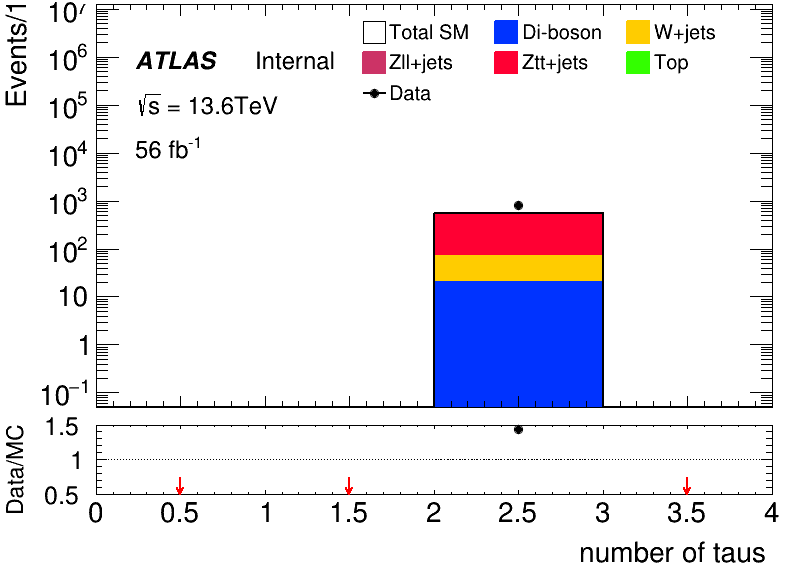
\includegraphics[width=0.20\textwidth]{graphics/HH_run3/HH_met_fb_nTaus.png} &
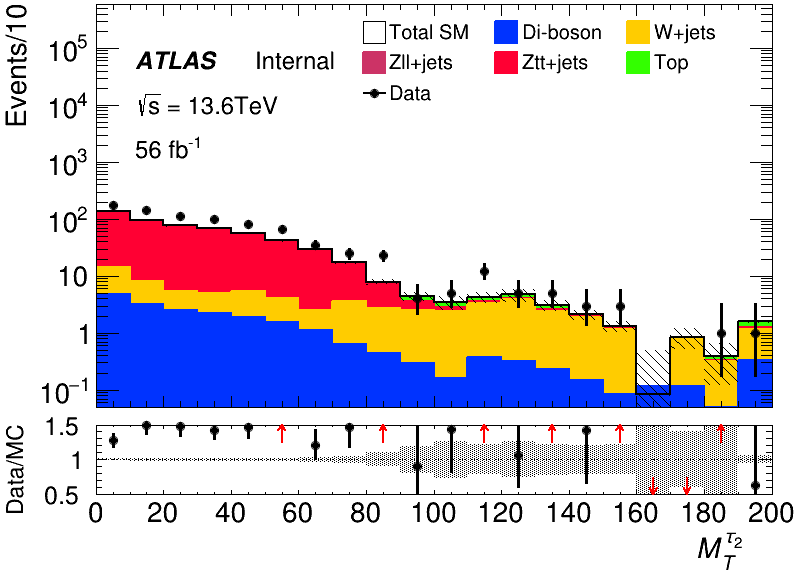
\includegraphics[width=0.20\textwidth]{graphics/HH_run3/HH_met_fb_mtx_tau2.png} &
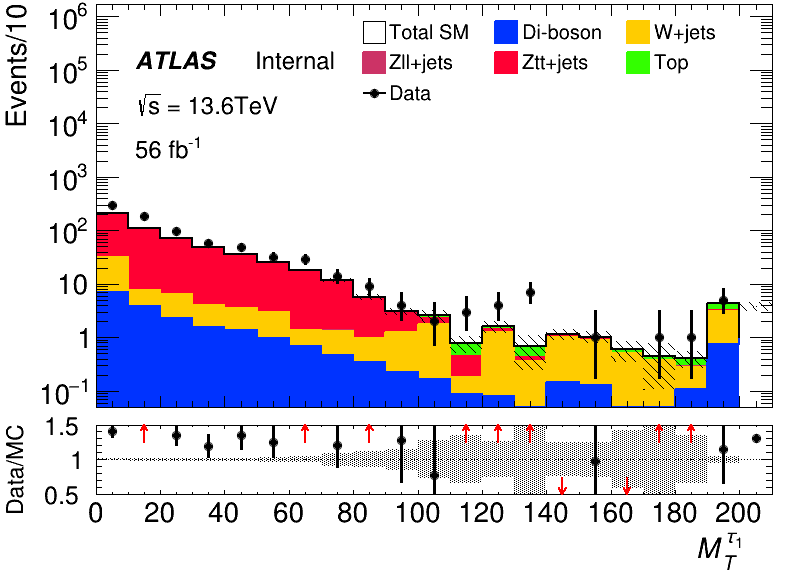
\includegraphics[width=0.20\textwidth]{graphics/HH_run3/HH_met_fb_mtx_tau1.png} \\
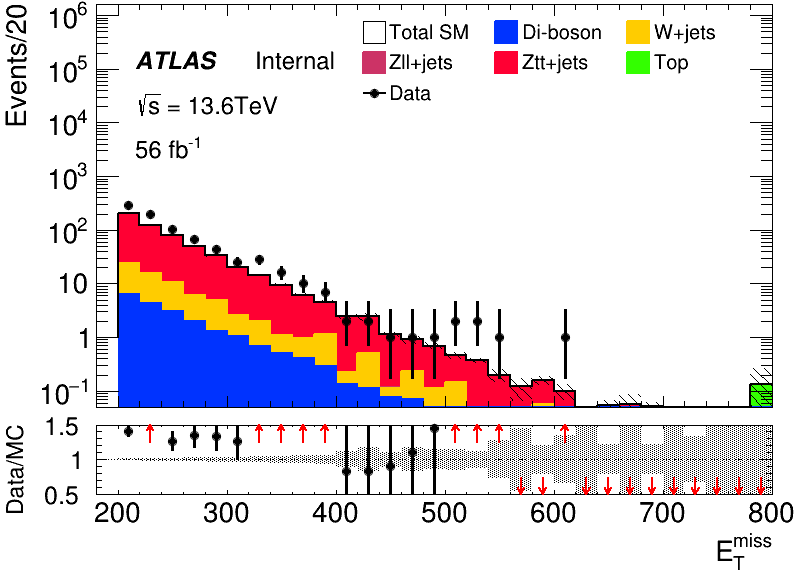
\includegraphics[width=0.20\textwidth]{graphics/HH_run3/HH_met_fb_MET.png} &
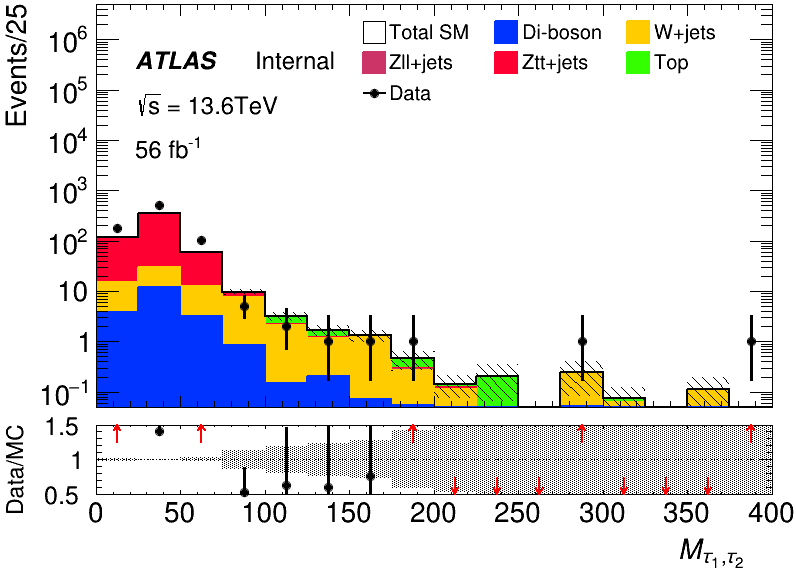
\includegraphics[width=0.20\textwidth]{graphics/HH_run3/HH_met_fb_Mll.png} &
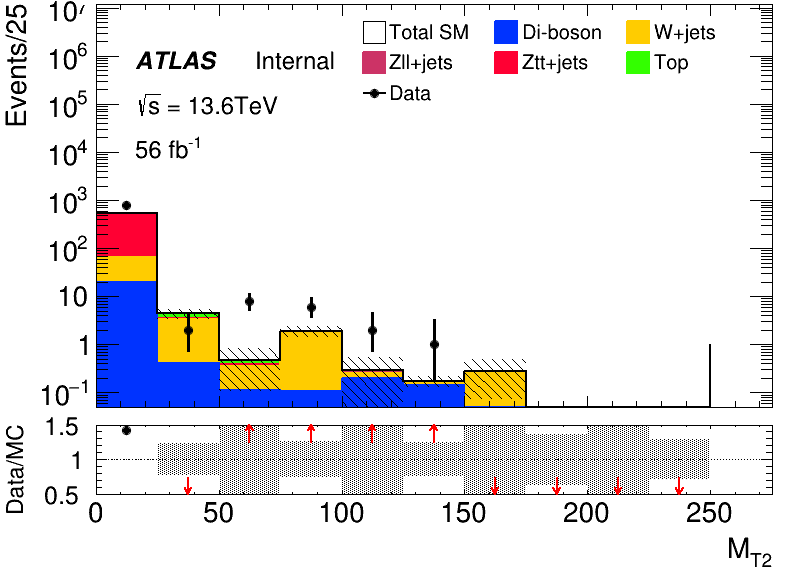
\includegraphics[width=0.20\textwidth]{graphics/HH_run3/HH_met_fb_MT2.png} &
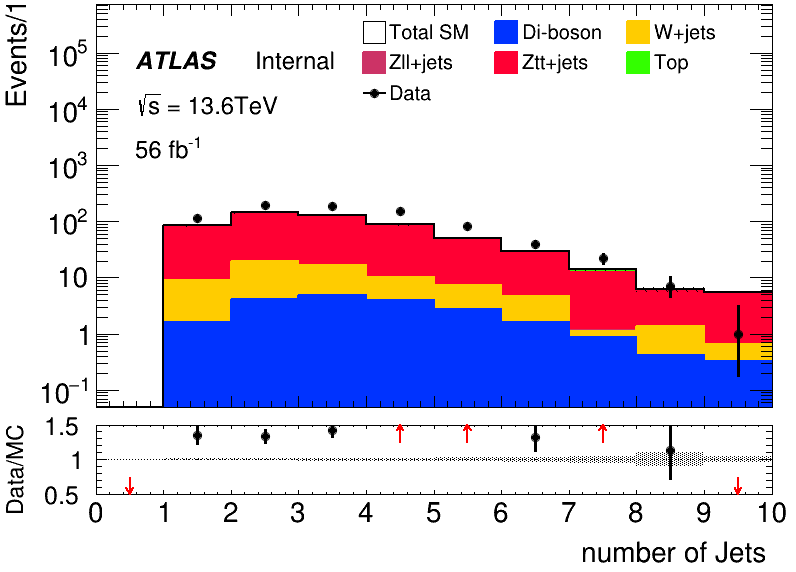
\includegraphics[width=0.20\textwidth]{graphics/HH_run3/HH_met_fb_nJets.png} &
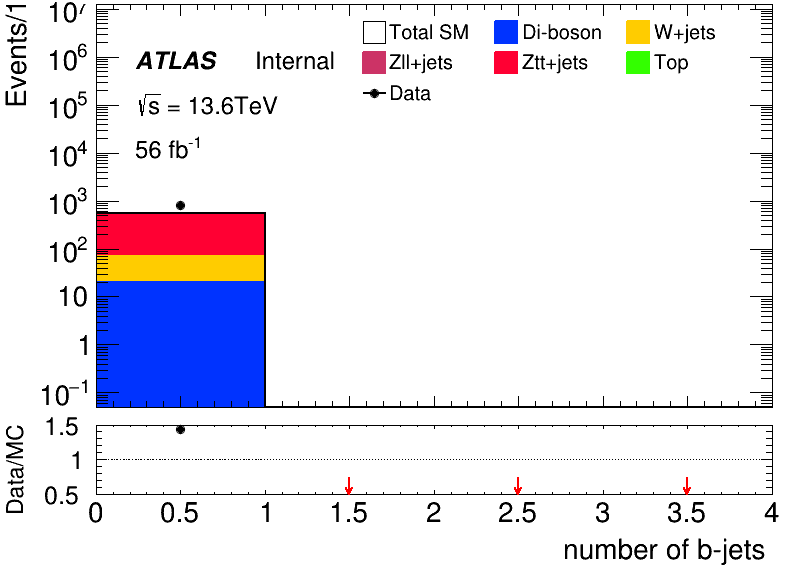
\includegraphics[width=0.20\textwidth]{graphics/HH_run3/HH_met_fb_bNumber.png} \\
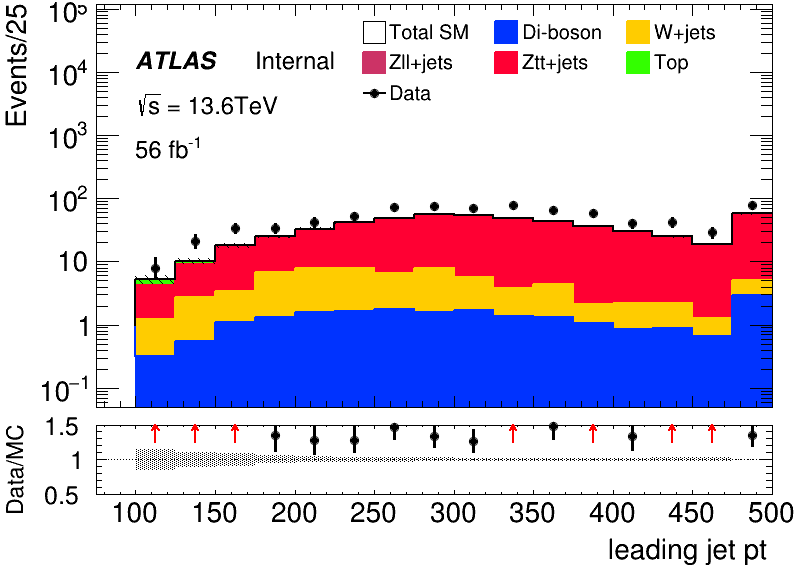
\includegraphics[width=0.20\textwidth]{graphics/HH_run3/HH_met_fb_pt_jet1.png} &
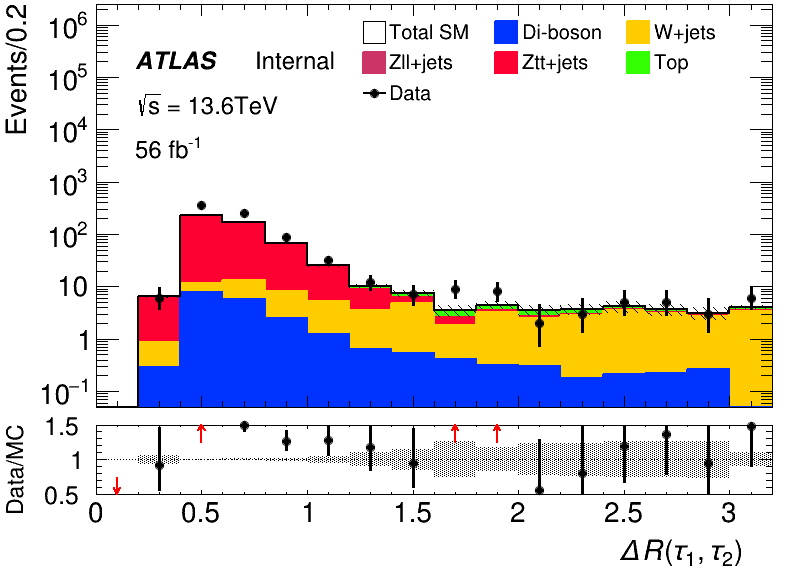
\includegraphics[width=0.20\textwidth]{graphics/HH_run3/HH_met_fb_dRtt.png} &
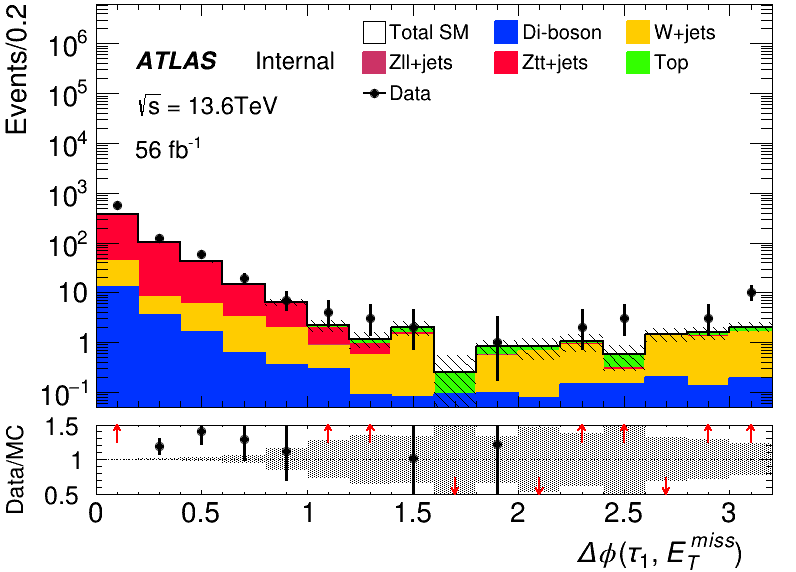
\includegraphics[width=0.20\textwidth]{graphics/HH_run3/HH_met_fb_dPhit1x.png} &
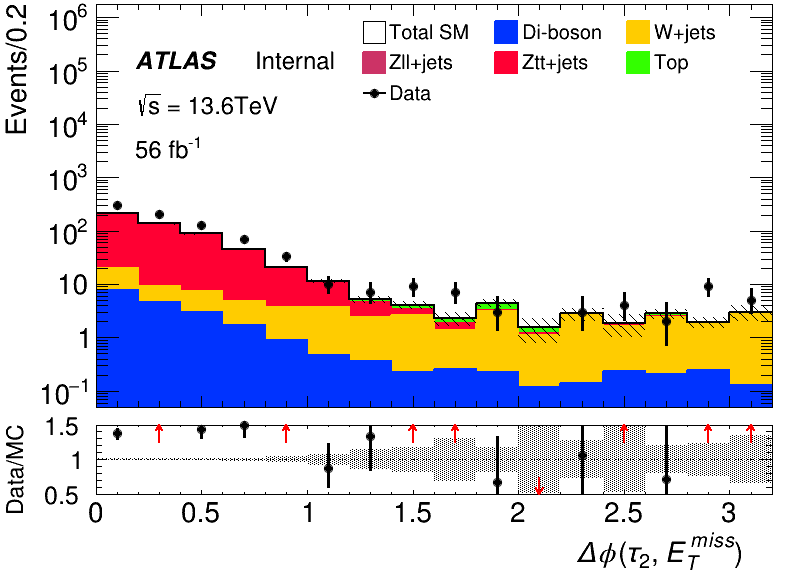
\includegraphics[width=0.20\textwidth]{graphics/HH_run3/HH_met_fb_dPhit2x.png} &
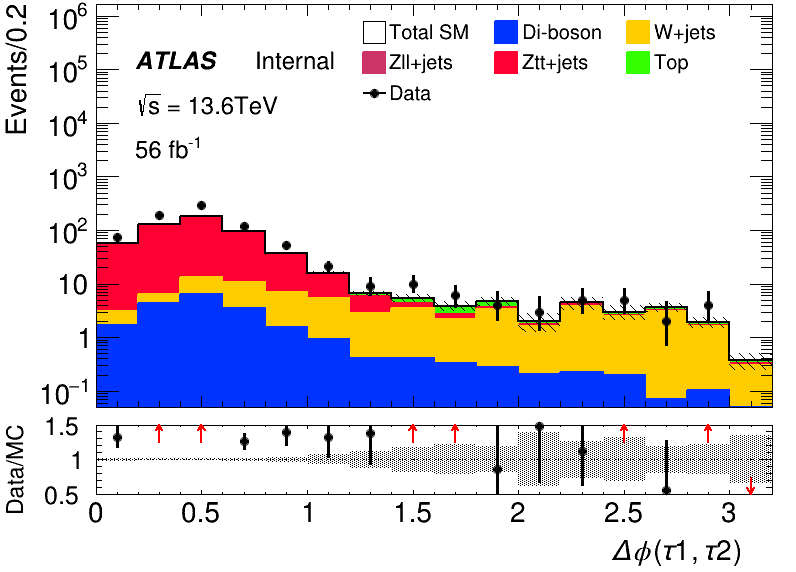
\includegraphics[width=0.20\textwidth]{graphics/HH_run3/HH_met_fb_dPhitt.png}
\end{tabular}
}

\end{frame}

\end{document}
 